% ===================================================
\section{Problem Statement}
% ===================================================
In this Part, we consider a two-agent pursuit-evasion problem that involves  a Target (aircraft) in opposition to an Attacker (missile). The Target tries to evade the Attacker and avoid being captured by him. We will try to find a simple technique for target evasion, so we should have a look at evasion techniques.
The missile is on the ground, its position is (0,0). The plane is flaying is the air, its position is (10000,40000).

\section{Evasion techniques}
There is some observations we should make before talking about evasion techniques 
\begin{itemize}
	\item The missile is faster than the aircraft, but cannot turn tighter than the aircraft, so it takes a longer path.
	\item The control mechanism of the Missile is much simpler and is of less capability than that of the aircraft. In order to pull as tight turn as the aircraft, it must exercise an acceleration that is far beyond its capability.
	\item The missile always attempts to trace the target. Thus if the target changes heading, it will necessary for the Missile to change heading similarly, but this is too difficult for him to achieve.
	\item  The main problem with evading missiles is their speed, which makes timing somewhat difficult.
\end{itemize}
\textbf{Some tactics to evade a missile:}
\begin{enumerate}
	\item \textbf{If missile is fired head-on at BVR range:}
	\begin{itemize}
		\item Turn hard to either left or right so as to fly at roughly 90 degrees angle to attacking aircraft (This forces missile to bleed off the energy and to lead the target).
		\item Once target aircraft makes a hard turn to reverse a direction, missile with its far larger turn circle – will be unable to compensate.
	\end{itemize}
					\begin{figure}[H]
					 	\centering
					 	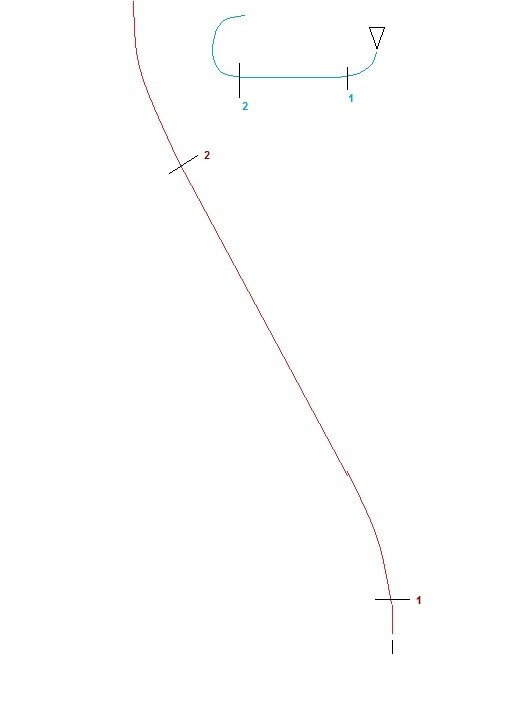
\includegraphics[scale = 0.25]{fig/evasiontech1.jpg}
					 	\caption{Illustration of the first maneuver technique}
					 	%\label{}
					 \end{figure}
	\item \textbf{ Jinking (useful at short ranges):}
	\begin{itemize}
		\item Aircraft must be positioned so that it is at angle (30-60 degrees is optimum) relative to missile’s flight path.
		\item Once missile gets closer, aircraft will make a hard turn in opposite direction.
		\item As there is a lag between aircraft changing the direction and missile following (for several reasons, most important of which is missile’s inertia), this will cause missile to head in wrong direction until it manages to correct, and also to bleed off the energy.
		\item Missile will fly past the aircraft and miss.
	\end{itemize}
					\begin{figure}[H]
						 \centering
						 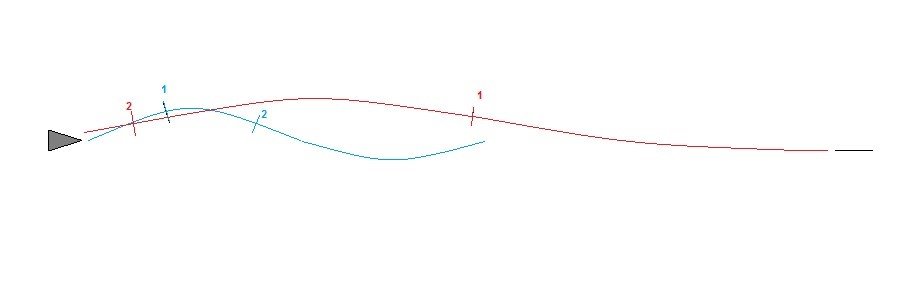
\includegraphics[scale = 0.7]{fig/evasiontech2.jpg}
						 \caption{Illustration of the second maneuver technique}
					\end{figure}
	\item  \textbf{Climb (useful at longer ranges):}
	\begin{itemize}
		\item Since at long range missile will have burned out its engine, it will rely on inertia to keep it flying, and climbing will mean that it will bleed off energy rapidly.
		\item Once missile reaches a close range (maybe around 1,500 meters), dive for the ground, then pull up (This will allow pilot to gain energy and using it to evade the missile).
	\end{itemize}
			\begin{figure}[H]
				\centering
				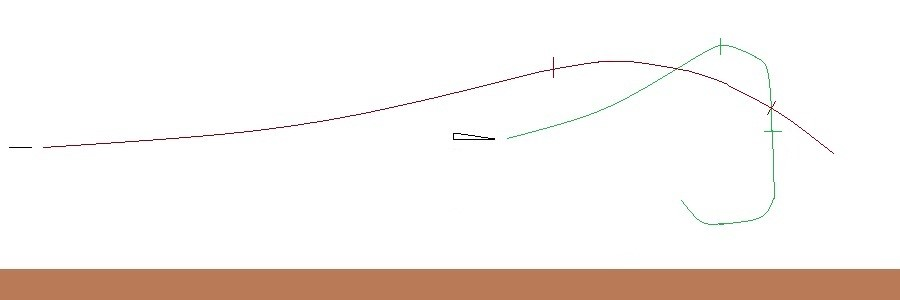
\includegraphics[scale = 0.7]{fig/evasiontech3.jpg}
				\caption{Illustration of the third maneuver technique}
			\end{figure}
	\item \textbf{Fourth tactic:}
	\begin{itemize}
		\item place the missile at 3 o’clock or 9 o’clock position
		\item maintain sufficient turn to keep the missile 
		\item This tactic forces the missile to execute a continuous turn, bleeding the energy entire time, making it easier to outturn the missile once it comes close.
	\end{itemize}
			\begin{figure}[H]
			\centering
			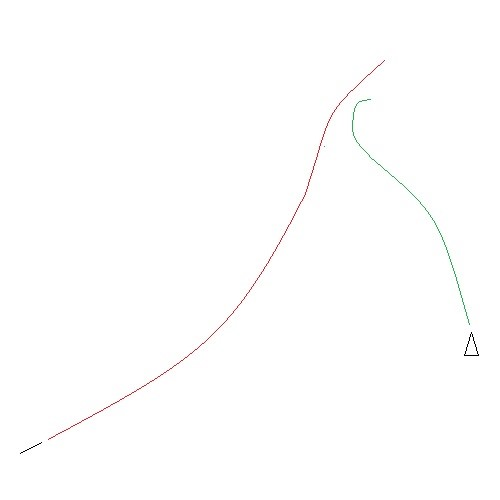
\includegraphics[scale = 0.7]{fig/evasiontech4.jpg}
			\caption{Illustration of the forth maneuver technique}
			\end{figure}
\end{enumerate}


%Why use polynomials?
Now we want to search for a path that the Target can move on it to escape from the Attacker. All the evasion techniques depend on the time of the turn that the Target makes when it detects the Attacker (Missile) and the objective is to maximize the Missile acceleration till the Missile power bleed. 
We will  choose the escaping trajectory as a polynomial with unknown coefficients, then try to find these coefficients which make the Missile exert a maximum acceleration to bleed its power as fast as we can before it reaches the Target.  
% ===================================================
\section{Assumptions, Notation, and Nomenclature}
% ===================================================
\subsection*{Assumptions}

\begin{enumerate}
	\item Both the Attacker and Target travel at constant speeds.
	\item The Attacker's speed is larger than that of the Target. Otherwise, the Target will be unconditionally or trivially capable of escaping. 
	\item Gravitational and drag effects are neglected for simplicity.
	\item The maximum g-force a typical person can handle is 5G
	\item The maximum g-force a pilot fighter (with safety equipments) could resist is 10G.
	\item The maximum g-force for a sprint missile is 100G.
	\item The range for Tactical missile defense, which has short ranges is $18\to 20$ Kilometer, approximately $59000 \to 66000$ feet. 
	
\end{enumerate}
% ===================================================

% ===================================================
\subsection*{Notation}
% ===================================================
\begin{itemize}
	\item $n_c$ : Acceleration command (for the Missile) in $m/s^2$.
	\item $N'$ : Effective navigation ratio, a unit-less designer-chosen gain (usually in the range of $3\to5$).
	\item $V_c$ : Missile-Target closing velocity.
	\item $\lambda$ : line-of-sight angle.
	\item $\dot{\lambda}$ : line of sight rate.
	\item $R_{TM}$ : length of the line of sight.
	\item $L$ : Missile lead angle.
	\item $HE$ : Heading error.
	\item $\dot{\beta}$ : angular velocity of the Target.
	\item $V_{T1},V_{T2}$ : Target velocity components in the Earth fixed coordinate system.
	\item $V_{M1},V_{M2}$ : Missile velocity components in the Earth fixed coordinate system.
\end{itemize}
% ===================================================
\subsection*{Nomenclature}

\textbf{Inertial coordinate system:} fixed to the surface of a flat-Earth model ( the 1 axis is downrange and the 2 axis can either be altitude or cross-range).

\textbf{Missile lead angle:} theoretically correct angle
for the missile to be on a collision triangle with the Target.

\textbf{Heading error ($HE$) :} angle representing the initial deviation of the Missile from the collision triangle.

\textbf{line of sight:} The imaginary line connecting the Missile and Target.

\textbf{length of the line of sight ($R_{TM}$):} Instantaneous separation between Missile and Target.

\textbf{Miss distance :} The point of closest approach of the Missile and Target.

\textbf{Closing velocity ($V_c$):} the negative rate of change of the distance
from the Missile to the Target $Vc= -\dot{R_{TM}}=-\frac{d}{dt} R_{TM} $.


% ===================================================
